\documentclass[a4paper,12pt,reqno]{article}
\usepackage{00}
\title{שפות תכנות}
\author{
יוסי גיל \\
הפקולטה למדעי המחשב⏎
הטכניון - מכון טכנולוגי לישראל⏎
}
\begin{document}
\maketitle
\section{הגדרות רקורסיביות}
§§ קבוצות מוגדרות רקורסיבית
סעיף 4ב' לחוק השבות, תש"י - 1950 קובע:
\צטט\ע|לענין חוק זה, "יהודי" - מי שנולד לאם יהודיה או שנתגייר, והוא אינו בן
דת אחרת|.===
נשים לב לכך כי בבואו להגדיר את המילה "יהודי", חוק השבות משתמש בגוף ההגדרה במילה
זו עצמה. הגדרות המשתמשות במונח המוגדר כחלק מההגדרה של המונח עצמו, נקראות הגדרות
רקורסיביות.

הגדרות רקורסיביות מופיעות גם בדתות אחרות: ע"פ השריעה (ההלכה המוסלמית), מוסלמי
הוא מי שנולד לאב מוסלמי או שהפך למוסלמי באמצעות אמירת העדות, הלא היא השהאדה:
\צטט
\begin{Arabic}
  \ע|اشهد ان لَا إِلٰهَ إِلَّا الله وان مُحَمَّدا رَسُولُ الله|
\end{Arabic}
===
(אני מעיד כי אין אלוהים לבד מאללה, וכי מוחמד הוא שליח אללה). בפני שלושה
מוסלמים. אנו רואים כי גם ההלכה המוסלמית מגדירה רקורסיבית את התשובה לשאלה "מיהו
מוסלמי?".

נאמר על קבוצה~$S$ שהיא מוגדרת באופן רקורסיבי (או בנוייה באופן רקורסיבי, או
לעיתים גם בנויה באופן אינדוקטיבי) אם ההגדרה של~$S$ מבדילה בין שני סוגים של
איברים: איברים אטומיים ואיברים מורכבים.
איברים מורכבים נוצרים באמצעות בנאי איברים מאיברים אטומיים ואיברים מורכבים
אחרים:
\begin{itemize}
  ✦ \ע|איברים אטומיים|. בסיס הרקורסיה הוא \ע|איברים אטומיים|, כלומר איברים
  של~$S$ אשר אינם נבנים מאיברים אחרים בקבוצה:
\ספרר
✦ אם נביט על סעיף 4ב' של חוק השבות כעח הגדרה רקורסיבית של קבוצת היהודים, סביר
שנאמר שאברהם אבינו ושרה
אמנו הם האיברים האטומיים של הקבוצה, כלומר הם יהודים בזכות עצמם.
✦ בהסתכלות דומה על השריעה, סביר להסיק מוחמד ואולי עוד כמה מתלמידיו, הם מוסלמים
מכוח עצמם בלבד.  כל שאר המוסלמים נקבעים בדרך אחרת.
===

✦ \ע|בנאי איברים|. הרקורסיה עצמנה נבנית באמצעות בנאי איברים, שהם כללים
המאפשרים לייצר איברים נוספים ל-$S$ מתוך איברים קיימים. איבר הנוצר על ידי בנאי
איברים, נקרא מורכב. בנאי איברים בונה איברים מורכבים של הקבוצה~$S$ מתוך איברים
אטומיים ואיברים מורכבים הקיימים בה. בהגדרה השרעית הרקורסיבית של קבוצות
המוסלמים יש שני בנאים:
\ספרר
✦ הבנאי שמאפשר לקבוע כי אדם מסויים הוא מוסלמי, אם אביו מוסלמי. בנאי זה הוא בנאי
אונארי, משום שבנאי זה מתחיל מאיבר יחיד בקבוצה (גבר שהוא מוסלמי), ומאפשר
"לבנות" איבר חדש מהאיבר הקיים.
✦ הכלל המגדיר כמוסלמי כמי שאמר את השהאדה בפני שלושה מוסלמים אחרים, הוא בנאי
טרנארי משום שבנאי זה מתסמך על שלושה איברים בקבוצה המוגדרת רקורסיבית (הלא היא
קבוצת המוסלמים), כדי לבנות איבר חדש בקבוצה.
===

גם חוק השבות מגדיר בנאי אונארי (אמהות). החוק אמנם אינו מגדיר
במדוייק מהו גיור, אך ברור כי הגדרה מדוייקת של הגיור, תכלול רקורסיה באמצעות בנאי
איברים ובפרט, ידרש כי חברי בית הדין המחליט על הגיור יהיו יהודים בעצמם.
\end{itemize}

\פסקה{הערות}
\החל{אבגוד}
✦ לעיתים נתייחס לאיברים האטומיים של קבוצה מוגדרת רקורסיבית כבנאים שהם nullary,
כלומר בנאים שאינם מקבלים ארגומנטים.
✦ גדלן של קבוצות המוגדרות רקורסיביות הוא בלתי חסום בדרך כלל, שכן תמיד ניתן
להשתמש בבנאים כדי ליצור איברים נוספים.
✦ קבוצה מוגדרת רקורסיבית יכולה להיות בעלת גודל סופי:
\ציינן
✦ אם הגדרת הקבוצה מכילה יחס שקילות, שגורים לכך שהפעלה אינסופית של בנאים, יוצרת
רק אוסף סופי של איברים שקולים.
✦ אם הבנאים אינם כאלו שתמיד ניתן להפעילם.
===
\סוף
{אבגוד}

הגדרה רקורסיבית מתאפייינת גם בתכונה נוספת:
\begin{itemize}
✦ \ע|שלמות ההגדרה|. הגדרה רקורסיבית של הקבוצה~$S$ כוללת תמיד בתוכה מרכיב
הדורש שאין ב-$S$ איברים אחרים מלבד האיברים האטומיים ואלו שנוצרו באמצעות בנאים.
בדרך הדרישה שבמרכיב זה של אינה נאמרת במפורש, אלא משתמעת מהניסוח. כך למשל מניסוח
חוק השבות, ברור כי ההגדרה מתכוונת לאמר שמי שאינו מקיים את התנאים המנויים בסעיף,
אינו יהודי. אך הקביעה כי כל מי שאמו אינו יהודיה ושלא התגייר איננו יהודי, אינה
מופיעה בחוק כלשונה אלא משתמעת ממנו.
\end{itemize}

§§ הגדרה רקורסיבית של קבוצת הפונקציות הרציונליות

נגדיר לדוגמה באופן רקורסיבי את~$ℚ₁$, קבוצת הפונקציות הרציונליות במשתנה אחד. כל
איבר~$f$ בקבוצה~$ℚ₁$ הוא פונקציה חלקית מ-ℝ (קבוצת המספרים הממשיים) אל~$ℝ$ .
כלומר~$f:ℝ⇸ℝ$. הכוונה במונח פונקציה חלקית היא שייתכן כי קיים ערך מסויים~$ℝ∈x$,
שעבורו ערך הפונקציה~\E|$f(x)$| אינו מוגדר. אנו נשתמש בסימון~$⊥$ כדי לציין את הערך
הלא מוגדר. ניתן לכן לכתוב~$f:ℝ→ℝ∪❴⊥❵$. בניסוח אחר,~$ℚ₁⊆ℝ⇸ℝ$, כלומר~$ℚ₁$ היא
קבוצה חלקית של קבוצת הפונצקיות החלקיות מ-$ℝ$ אל~$ℝ$.

\החל{definition}\label{definition:rationals}
הקבוצה ב-$ℚ₁$, קבוצת הפונקציות הרציונליות במשתנה אחד, מוגדרת על ידי שלושת
התנאים הבאים:
\begin{enumerate}
✦ \ע|איברים אטומיים של קבוצת הפונקציות הרציונליות|
\begin{itemize}
✦ הפונקציה~$U$, המעתיקה כל מספר ממשי אל המספר הטבעי~$1$,
\begin{equation*}
  ∀ x∈ℝ∙ U(x)=1,
\end{equation*}
נמצאת בקבוצה~$ℚ₁$,
כלומר
\begin{equation}\label{eq:1}
  U∈ℚ₁
\end{equation}
✦ פונקצית הזהות,~$I$, המעתיקה כל מספר ממשי אל עצמו,
\begin{equation*}
  ∀ x∈ℝ∙ I(x)=x
\end{equation*}
נמצאת בקבוצה~$ℚ₁$, כלומר
\begin{equation}\label{eq:x}
  I∈ℚ₁
\end{equation}
\end{itemize}
✦ \ע|בנאים של קבוצת הפונקציות הרציונליות|
\begin{itemize}
✦ אם הפונקציה~$f$ שייכת ל-$ℚ₁$ אזי גם הפונקציה~$-f$ שייכת לקבוצה זו, כלומר
\begin{equation}\label{eq:minus}
  -f∈ℚ₁.
\end{equation}
✦ אם שתי הפונקציות~$f₁$ ו-$f₂$ שייכות ל-$ℚ₁$ אזי גם הסכום שלהן, המכפלה
שלהן, והמנה שלהן שייכות ל-$ℚ₁$, כלומר
\begin{align}
  f₁+f₂ &∈ℚ₁, \label{eq:plus} ⏎
  f₁·f₂ &∈ℚ₁ \label{eq:times} ⏎
  f₁/f₂ &∈ℚ₁. \label{eq:div}
\end{align}
\end{itemize}
✦ \ע|שלמות ההגדרה: אין פונקציות רציונליות חוץ מהאטומיות ואלו שנוצרו באמצעות
הבנאים| ⏎ 
הקבוצה~$ℚ₁$ היא הקבוצה הקטנה ביותר של פונקציות המקיימת את התנאים
\פנה|eq:1|,
\פנה|eq:x|,
\פנה|eq:minus|,
\פנה|eq:plus|,
\פנה|eq:times|
ו-\פנה|eq:div|.
\end{enumerate}
\סוף{definition}

§§ כתיב של כללי היסק

ניסוח תמציתי ומדוייק לבנאים הוא ככללי היסק \E|(inference rules)| כפי שהם נהוגים
בתחשיב הפסוקים. כלל היסק האומר שבכל פעם שמתקיימות ההנחות~$P₁,P₂,…,Pₙ$ ניתן
להסיק את המסקנה~$Q$ יכתב כך: \[
  \dfrac{\begin{array}{c}P₁ ⏎P₂ ⏎⋮ ⏎Pₙ\end{array}}{Q}
\] ניתן גם לכתוב את הדרישות בשורה אחת, ובלבד שהן מופרדות זו מזו, \[
  \infer Q{P₁ & P₂ &⋯& Pₙ}
\] לדוגמה, את הבנאי \פנה|eq:plus| של הקבוצה~$ℚ₁$, ניתן לכתוב ככלל היסק:
\begin{equation*}
  \infer{f₁+f₂∈ℚ₁}{f₁∈ℚ₁ & f₂∈ℚ₁}
\end{equation*}
בכלל היסק זה יש שתי הנחות~$P₁=f₁∈ℚ₁$ ו-$P₂=f₂∈ℚ₁$. כל אחת מההנחות צריכה להיקרא
ככמת אוניברסלי כפי שהוא מופיע בתחשיב הפסוקים, כלומר, עבור כל בחירה של
פונקציה~$f₁$ המקיימת~$f₁∈ℚ₁$ ולכל בחירה של פונקציה~$f₂$ המקיים~$f₂∈ℚ₁$ נובעת
המסקנה~$Q=f₁+f₂∈ℚ₁$. בניסוח אחר כלל ההיסק אומר כי \[
  ∀f₁∀f₂❨f₁∈ℚ₁∧f₂∈ℚ₁→f₁+f₂∈ℚ₁❩.
\] ניתן לנסח את ארבעת הבנאים של הקבוצה~$ℚ₁$, כלומר \פנה|eq:minus|,
\פנה|eq:plus|,
\פנה|eq:times|
ו-\פנה|eq:div|,
ככלל היסק אחד:
\begin{equation*}
  \infer{-f₁,f₁+f₂, f₁·f₂,f₁/f₂∈ℚ₁}{f₁∈ℚ₁&f₂∈ℚ₁}
\end{equation*}

ניתן גם לנסח את הגדרת האיברים האטומיים של הקבוצה~$ℚ₁$, כלומר \פנה|eq:1|
ו-\פנה|eq:x|,
כשני כללי היסק אשר קבוצת ההנחות שלהן ריקה,
\begin{equation*}
  \begin{array}{ccc}
    \infer{I∈ℚ₁}{} & & \infer{1∈ℚ₁}{}
  \end{array}\hfill
\end{equation*}
או בקיצור, ככלל אחד,
\begin{equation*}
  \infer{1, I∈ℚ₁}{}
\end{equation*}
לדוגמה, \[
  \frac {I+1}{I·I -3·I+1}
\] הוא איבר ב-$ℚ₁$,
שמיייצג את הפונקציה~$f(x)=(x+1)/(x²-3x+1)$.

ניתן להשתמש במבנה ההגדרה הרקורסיבי של קבוצה בהגדרות רקורסיביות נוספות המתייחסות
לקבוצה ולאיבריה.

\begin{definition}[ערך של פונקציה רציונלית]
עבור פונקציה רציונלית~$f∈ℚ₁$, ועבור כל מספר ממשי~$x∈ℝ$ נגדיר את~$f(x)$
רקורסיבית
\begin{equation}\label{eq:value}
  \begin{array}{cc}
    U(x)=1 & I(x)=x ⏎ ⏎
    \infer{-f(x)=-x₁}{f(x)=x₁} & \infer{(f₁+f₂)(x)=x₁+x₂}{f₁(x)=x₁ & f₂(x)=x₂} ⏎ ⏎
    \infer{(f₁·f₂)(x)=x₁·x₂}{f₁(x)=x₁ & f₂(x)=x₂} &
    \infer{(f₁/f₂)(x)=x₁/x₂}{f₁(x)=x₁ & f₂(x)=x₂}
  \end{array}
\end{equation}
\end{definition}

§§ אינדוקצית מבנה
הגדרות רקורסיביות מאפשרות לנו להוכיח טענות באינדוקציה הידועה בשם אינדוקצית
מבנה. באינדוקציה כזו, אנו מוכיחים ראשית כי הטענה נכונה עבור כל האיברים האטומיים
של קבוצה. בצעד האינדוקציה נעבור על כל בנאי האיברים: לגבי כל בנאי נניח שהטענה
נכונה לגבי כל האיברים עליהם פועל, ונוכיח כי הטענה נכונה גם עבור האיבר אשר אותו
יצר הבנאי. ניתן גם להסתכל על הוכחות באינדוקצית מבנה כאינדוקציה על מספר
ההפעלות~$n$ של בנאים לשם יצירת~$f$.

נוכיח לדוגמה את הטענה הפשוטה הבאה עבור ההגדרה הרקורסיבית של הקבוצה~$ℚ₁$
(\פנה|definition:rationals|) וההגדרה של ערך הפונקציה מעל \פנה|eq:value|.

\begin{claim}
  עבור כל מספר רציונלי~$q∈ℚ$, ועבור כל פונקציה רציונלית~$f∈ℚ₁$, מתקיים כי
  \begin{equation}\label{eq:Q}
    f(q)∈ℚ∪❴⊥❵
  \end{equation}
  כלומר~$f(q)$ אינו מוגדר, או שהוא מספר רציונלי.
\end{claim}

\begin{proof}
  \mbox{}
  \תאר
  ✦ [בסיס האינדוקציה] אם~$n=0$ אז~$f$ הוא איבר אטומי של~$ℚ₁$,
  ואז~$f=1$ או~$f=I$ וברור שאם~$q$ רציונלי, אז גם~$f(q)∈❴1,q❵$. ולכן
  \פנה|eq:Q| מתקיימת עבור~$n=0$.
  ✦ [צעד האינדוקציה] נניח שהטענה \פנה|eq:Q| מתקיימת עבור כל~$n'$, כאשר~$n'<n$
  ונוכיח אותה עבור~$n$.
  נסתכל על איבר~$f∈ℚ₁$ אשר נוצר מהפעלה של~$n$ בנאים, ונניח ש-$n>0$ כלומר~$f$
  נוצר על ידי הפעלה של בנאי. בנאי זה הוא אחד מארבעת הבנאים \פנה|eq:minus|,
  \פנה|eq:plus|, \פנה|eq:times|, או \פנה|eq:div|.
  מכאן, \[
    f(q)∈❴-q₁,q₁+q₂,q₁·q₂,q₁/q₂❵.
  \] כיוון שמספר הפעולות הבנאים לשם יצירת הפונקציות~$f₁$ ו-$f₂$ קטן ממש מ-$n$
  הנחת האינדוקציה מתקיימת לגביהן, ולכן, גם~$q₁$ וגם~$q₂$ חייבים להיות רציונליים
  אם הם מוגדרים, ולכן גם~$f(q)$, אם הוא מוגדר, חייב להיות מספר רציונלי.
 ===
\end{proof}

הגדרות רקורסיביות משמשות לעיתים קרובות באיפיון של שפות תכנות. אוסף הביטויים
המותר לשימוש בשפה, אוסף הפקודות, ואוסף הטיפוסים, כמעט תמיד מוגדרים רקורסיבית.

§§ הגדרה רקרוסיבית של ביטויים בשפות תכנות

בשפת \פסקל הביטוי
\begin{PASCAL}
(-12+sin(13.4)) * x
\end{PASCAL}
הוא ביטוי מורכב המכיל בתוכו שלושה ביטויים אטומיים \קד{12}, \קד{13.4}
ו-\קד{x}. בביטוי מופיע הבנאי הבינארי של החיבור, הבנאי הבינארי של הכפל,
ושלושה בנאים אונאריים: סימן המינוס החד מקומי (\קד{-$·$}), הפונקציה החד מקומית
\קד{sin($·$)}, וגם בנאי אונארי נוסף המאפשר לעטוף ביטוי בסוגרים. על פי בנאי
זה, אם~$E$ הוא ביטוי אזי גם \קד{($E$)} הוא ביטוי, ועל כן, כיוון
ש-\קד{-12+sin(13.4)} הוא ביטוי אזי גם \קד{(-12+sin(13.4))} הוא ביטוי.

כל הגדרה רקורסיבית של קבוצת הביטויים המותרים לשימוש בשפת תכנות מסויימת, כוללת
קביעה מי הם הביטויים האטומיים, כלומר ביטויים שאינם מכילים בתוכם ביטויים אחרים.
בדרך כלל ביטויים האטומיים הם משני סוגים: ליטרלים כגון המספר השלם \קד{21} והמספר
הממשי \קד{13.4} ושמות, כגון \קד{x}. השיערוך של ביטוי מוגדר רקורסיבית. השיערוך
של ליטרל, הוא ערכו של הליטרל, ואילו שיערוך של שם נעשה באמצעות חיפוש השמות של
הערך המתאים לשם.

מלבד הביטויים האטומיים, ההגדרה הרקורסיבית של קבוצת הביטויים המותרים לשימוש,
כוללת בתוכה גם רשימה של בנאי ביטויים. בנאי ביטויים אונארי המופיע כמעט בכל שפת
תכנות נפוץ הוא זוג סוגריים: אם~$E$ הוא ביטוי, אזי גם~$⌘)E⌘($ הוא ביטוי.
גם אופרטורים הם בנאי ביטויים נפוצים: אופרטורים אונאריים, כגון סימן המינוס החד
מקומי (\קד-) הם בנאי ביטויים אונאריים, שכן, אם~$E$ הוא ביטוי,
אזי גם~$⌘-E$ הוא ביטוי. אופרטורים בינאריים, כגון החיבור (קד+) והכפל (\קד*) הם
בנאי ביטויים בינאריים, שכן אם~$E₁$ ו-$E₂$ הם ביטויים אזי גם~$E₁⌘+E₂$
ו~$E₁⌘*E₂$ הוא ביטוי. בשפת התכנות~\E|\CPL|, כמו גם שפות תכנות אחרות, יש גם
אופטור טרנרי, על פיו אם~$E₁$,~$E₂$ ו-$E₃$ הם ביטויים אזי גם
$E₁⌘?E₂⌘:E₃$ הוא ביטוי.

בנאי הביטויים כוללים בתוכם גם פונקציות. אם~$⌘f$ היא פונקציה~$n$-מקומית עבור
ו-$E₁,E₂,…,Eₙ$ הם ביטויים אזי גם~$⌘f⌘)E₁⌘,E₂⌘,…⌘,Eₙ⌘($ הוא ביטוי.  מקרה מעניין
הוא זה שבו~$n=0$. פונקציה 0-מקומית יוצרת היא בנאי \E|nullary|, שיוצרת ביטוי
אטומי ללא שימוש בביטויים אחרים.  בשפת~\E|\CPL|, הכתיב~$⌘{f()}$ המשמש לקריאה
לפונקציה ללא ארגומנטים, מטעים שפונקציה זו מהווה בנאי \E|nullary|.  בשפת פסקל,
הכתיב~$⌘f$ המשמש לקריאה לפונקציה כזו מטעים שפונקציה זו היא ביטוי אטומי.

האבחנה שגם אופרטורים וגם פונקציות הם בנאי ביטויים, מאפשרת לנו לזהות שהההבדל
ביניהם הוא דקדוקי יותר מאשר עקרוני:

\החל{אבגוד}
✦ אופרטורים נכתבים בדרך כלל בכתיב של \E|infix|, כלומר, בין הארגומנטים שלהם.
אופרטורים אונאריים יכולים להיכתב בכתיב של \E|prefix|, כלומר לפני הארגומנט שלהם,
או בכתיב של \E|postfix|, כלומר אחרי הארגומנט שלהם. לעומת זאת, פונציות נכתבות
תמיד בכתיב של \E|prefix|.
הביטוי הבא בשפת C מדגים אופרטרים הכתובים ב-\E|prefix|, \E|postfix|, ו-\E|infix|,
ופונקציות בנות 0, 1, ו-3 ארגומנטים הכתובות כולן ב-\E|postfix|.
\begin{CPP}
     g(a) ? f(++a,b++,h()) : a+b
\end{CPP}
✦ פונקציות המקבלות ארגומנט אחד או יותר נכתבות תמיד עם סימני סוגריים, ולכן, יש
רק דרך אחת לפרש ביטוי שבו הבנאים היחידים הם פונקציות.

לעומת זאת, אורפטורים נכתבים בדרך כלל ללא סוגריים. סדר הקדימויות של האופרטורים
הוא זה הקובע את מבנה הביטוי. הכתיב של אופרטורים קצר יותר, אך גם מחייב
שימוש בסימני סוגריים כדי להתגבר על סדר הקדימויות.

✦ השמות של פונקציות נראים בדרך כלל כמו "שמות רגילים", הכוללים בתוכם אותיות
אנגליות, ולעיתים גם ספרות, וסימנים מפרידים. לעומת זאת, שמות האופרטרים הם בדרך
כלל סדרה של סימני פיסוק. בכל זאת, ישנן שפות רבות בהן לפחות למקצת האופרטורים יש
שמות שהם מילים. למשל, שמו של האופרטור~$∧$, בשפת פסקל, הוא המילה
השמורה~$⌘{and}$.

מצד שני, קיימות שפות תכנות בהן ניתן לתת לפונקציות שמות המורכבים מסימני פיסוק
בלבד.

✦ אופרטורים בדרך כלל מוגדרים על ידי שפת התכנות, בעוד שפונקציות מוגדרות על ידי
  המתכנת. יחד עם זאת, ישנן שפות תכנות רבות המאפשרות למתכנת להגדיר אופרטורים
  חדשים שאינם מוכרים על ידי השפה. ומנגד, ישנן שפות תכנות שבהן ישנן פונקציות
  המוגדרות על ידי השפה, ולא על ידי המשתמש.
\סוף{אבגוד}

§§ פקודות
לבד מביטויים, תכניות גם מכילות פקודות אשר ביצוען מביא לשינוי של מצב התכנית. גם
גם קבוצת הפקודות מוגדרת בדרך כלל רקורסיבית, והגדרה זו כוללת בתוכה
הגדרה של בנאי פקודות ופקודות אטומיות.

פקודה אטומית יכולה להכיל בתוכו ביטוי, והביטוי יכול שיהיה ביטוי מורכב, גם אם
הפקודה עצמה היא אטומית.
לדוגמה, בשפת פסקל, פקודות אטומיות מכילות גם את פקודת ההצבה. כך,
\begin{PASCAL}
x:=(-12+sin(13.4))*x
\end{PASCAL}
היא פקודה אטומית שבה מחושב ערכו של הביטוי \קד{(-12+sin(13.4))*x},
ולאחר החישוב, הערך מוצב אל תוך המשתנה \קד{x}.
בפקודה זו נוכל לזהות תתי מרכיבים: למשל תת-הביטוי \קד{sin(13.4}.
 בכל זאת, הפקודה היא פקודה אטומית, שכן לא ניתן לזהות בה תת-מרכיב שהוא \פקודה
 בעצמו. באופן כללי יותר, איבר מקבוצה המוגדרת רקורסיבית הוא איבר אטומי אם
לא ניתן לזהות בתוכו תת-איבר אחד או יותר השייך לאותה קבוצה. אבל איבר אטומי אינו
בהכרח לא פריק: האטומיות נובעת מכך שלא כל שנדרש הוא שלא ניתן לזהות בתוכה תת-איבר
מאותה קבוצה.

לבד מהצבה, בשפת התכנות פסקל ישנן פקודות אטומיות משלושה סוגים נוספים:
\begin{enumerate}
✦ \ע|קריאה לפרוצדורה|. זוהי פקודה כגון
\begin{PASCAL}
WriteLn('Hello, World')
\end{PASCAL}
אשר קוראת לפרוצדורה המוגדרת בשפה, או פרוצדורה המוגדרת על ידי המתכנת, כמו
\begin{PASCAL}
ComputeSolution(1,5,6,x)
\end{PASCAL}
✦ \ע|פקודת קפיצה|. זוהי פקודה כגון
\begin{PASCAL}
goto 999
\end{PASCAL}
אשר בה בקרת הזרימה מועברת למקום אחר בתכנית. בדוגמה שלנו, הפקודה המסומנת בתגית
999.
✦ \ע|הפקודה הריקה|. זוהי פקודה שאינה עושה דבר. אין צורך לכתוב דבר כדי
להשתמש בפקודה זו, והיא משמשת בעיקר לצורך בניית פקודות מורכבות
\end{enumerate}
בשפת פסקל יש גם בנאי פקודות. החשובים ביותר הם אלו:
\begin{enumerate}
✦ \ע|בנאי הבלוק|. סדרה של פקודות המופרדות על ידי סימן הנקודה ופסיק (\קד{;|)
והעטופה במילים \מש{begin} ו\מש{end} גם היא פקודה. בנאי הבלוק הוא בנאי רב
מקומי, שיכול לקבל מספר כלשהו של פקודות, מורכבות או אטומיות, ולבנות מהם פקודה
אחת. זו לדוגמה פקודה מורכבת הנוצרת על ידי בנאי הבלוק משתי פקודות אטומיות.
\begin{PASCAL}
begin
  a:=b;
  goto 999
end
\end{PASCAL}
נשים לב לכך שסימן הנקודה ופסיק (\קד{;}) מפריד בין פקודות ואינו חלק מהפקודה.
לכן,
\begin{PASCAL}
begin
  a:=b;
  goto 999;
end
\end{PASCAL}
היא פקודה מורכבת הנוצרת משלוש פקודות אטומיות, שהאחרונה בהן ריקה. בנאי הבלוק הוא
גם \E|nullary|, וגם 
\begin{PASCAL}
begin
end
\end{PASCAL}
היא פקודה.
✦ \ע|בנאי לולאת ה-\קד{while}}. בנאי לולאת ה-\קד{while| הוא בנאי אונארי:
אם~$C$ היא פקודה ו-$E$ הוא ביטוי בוליאני, אזי גם לולאת ה\קד{while}
\begin{PASCAL}
while ⌘$E$⌘ do ⌘$C$⌘
\end{PASCAL}
היא פקודה. על פי בנאי זה,
\begin{PASCAL}
while x > sin(x) do x :=sin(x)
\end{PASCAL}
✦ \ע|בנאי התנאי החלקי|. גם בנאי התנאי החלקי הוא בנאי אונארי. לפי בנאי זה,
אם~$C$ היא פקודה ו-$E$ הוא ביטוי בוליאני, אזי גם פקודת התנאי החלקי היא פקודה:
\begin{PASCAL}
if ⌘$E$⌘ then ⌘$C$⌘
\end{PASCAL}
✦ \ע|בנאי התנאי המלא|. אם~$C₁$ ו-$C₂$ הן פקודות ו-$E$ הוא ביטוי בוליאני, אזי
גם פקודת התנאי המלא היא פקודה:
\begin{PASCAL}
if ⌘$E$⌘ then ⌘$C₁$⌘ else ⌘$C₂$⌘
\end{PASCAL}
היא פקודה.
\end{enumerate}

קבוצת הפקודות במרבית שפות התכנות היא קבוצה המוגדרת רקורסיבית, ובתוך קבוצה זו,
אנו יכולים לזהות את הפקודות האטומיות. אולם, כפי שנראה, לעומת זאת, הפקודה הבאה
בפסקל,
\החל{PASCAL}
begin
c :=a;
a :=b;
b :=c;
end
\end{PASCAL}
אינה פקודה אטומית, שכן ניתן לאתר בה מרכיב שהוא \פקודה בעצמו.

§§§ טיפוסים
במרבית שפות התכנות, קבוצת הטיפוסים בהם ניתן להשתמש בשפה, גם היא מוגדרת
רקורסיבית. לדוגמה, מערכת הטיפוסים בשפת התכנות \E|Nִִִim|, ניתן לתיאור רקורסיבי
פשוט: 
\begin{description}
✦ [טיפוסים אטומיים] אלו הם טיפוסים שאינם מורכבים משום טיפוס אחר.  אחדים
מטיפוסים אלו הם טיפוסים מוגדרים מראש בשפת \E|Nim|.
\begin{description}
✦ {טיפוסי מספר שלם:}
אלו כוללים את הטיפוסים
\E|int|, int8, int16, int32, ו-int64,
כמו גם את הגירסאות חסרות הסימן של טיפוסים אלו:
\E|uint|, uint8, uint16, uint32, ו-uint64.
✦ {טיפוסי מספר ממשי:} הכוללים בתוכם את הטיפוסים float, float32, ו-float64.
✦ {הטיפוס char :} הכוללים בתוכם את הטיפוסים float, float32, ו-float64.
:
והם מכילים בתוכם את הטיפוסים הבאים:
\end{description}
✦ [בנאי טיפוסים] אלו הם טיפוסים שאינם מורכבים משום טיפוס אחר.
\end{description}

קבוצת ה\טיפוסים שֶׁל שפת \סי (כמו גם קבוצת הטיפוסים שֶׁל שפת פסקל) אף היא קבוצה
המוגדרת רקורסיבית: ישנם טיפוסים מורכבים, אשר ניתן לזהות כי הם מורכבים מיחידות
קטנות יותר, אשר אף הן טיפוסים. בטיפוס רשומה למשל ניתן לזהות כיחידות קטנות יותר
את טיפוסי השדות הבונים את הרשומה. אנו אומרים שהטיפוס שֶׁל רשומה הוא טיפוס
מורכב, משום שיש בו תתי-יחידות אשר אף הן טיפוסים.

לעומת הטיפוסים המורכבים, ישנם טיפוסים אטומיים, כלומר טיפוסים אשר לא ניתן לזהות
בתוכם טיפוסים אחרים. הטיפוס שֶׁל מספרים שלמים או הטיפוס שֶׁל מספרים ממשיים, הם
דוגמאות לטיפוסים כאלו.

המילה השמורה \מש{int} בשפת \סי \מזהה את הטיפוס האטומי שֶׁל מספר שלם. מילים
שמורות המשמשות כ\מזהים נקראות מזהה שמור.

ניתן להשתמש בשיטת ההגדרה הרקורסיבית, כדי להגדיר את קבוצת הפקודות בפסקל,

\begin{enumerate}
✦ \ע|פקודות אטומיות| פקודות אטומיות הן פקודות שאינן בנויות מפקודות אחרות. בשפת
\סי יש שני סוגים של פקודות אטומיות, 
\begin{enumerate}
✦ \ע|פקודה ריקה| פקודה שאינה מבצעת דבר, נקראת הפקודה הריקה. הפקודה הריקה נכתבת
בשפת אמצעות סימן הנקודה ופסיק~\cc{;}.
✦ \ע|פקודת ביטוי| בשפת \סי, כל ביטוי שאחריו מופיע סימן הנקודה ופסיק~\cc{;|}
\begin{CPP}
  a; f(); b=2; 2;++i; 1-1;
\end{CPP}
\end{enumerate}
קריאה לפרוצדורה
כללי היצירה העיקריים של הפקודות הם:
שרשור של פקודות המופרדות על ידי סימן הנקודה ופסיק (;) הוא פקודה.
פקודת תנאי, כפי שתוארה לעיל, היא פקודה, אשר מכילה בתוכה פקודה אחת או שתיים.
פקודת תנאי רבת ראשים המוגדרת באמצעות המילה השמורה case
לולאות המתארות ביצוע איטרטיבי של פקודה (אטומית או מורכבת), אף הן פקודות. יש
בְּPascal שלושה סוגים של פקודות לולאה מורכבות: for
while
repeat until
\end{enumerate}
\end{enumerate}

string, char, ו-bool,
וכו', וישנם בנאי טיפוסים המאפשרים להגדיר טיפוסים מורכבים מתוך טיפוסים
סוף{ציינון}

מערכים בִּשְׂפַת Pascal הם טיפוסים מורכבים: בנאי המערך קיבל כפרמטר את טיפוס של תא
במערך, והחזיר בתמורה את טיפוס המערך של תאים מאותו טיפוס.†{למען השלמות יש לציין
שבנאי המערך מקבל עוד שני פרמטרים, שהם קצוות המערך. ואפשר להפליג ולצין שבנאי של
מערך רב מימדי מקבל מספר זוגות של פרמטרים כנ"ל.}
איבר אטומי הוא איבר שנוצר מבנאי שלא קיבל כפרמטרים ערכים של הקבוצה.

ניתן להסתכל על הטיפוסים אטומיים מכוח עצמם: Character, Integer, Real, Boolean
כעל בנאים שאינם מקבלים פרמטרים כלל. טיפוסים מנויים (enumerated types) בִּשְׂפַת
פסקל, הם גם טיפוסים אטומיים (איברים אטומיים של קבוצת הטיפוסים) . הם נוצרו מבנאי
שמקבלל רשימה של תגיות. תגית היא מזהה חוקי בִּשְׂפַת פסקל.

\section{שפות פורמליות}
אלפאבית הוא קבוצה, בדרך כלל סופית, של איברים הקרויים אותיות או סמלים. לדוגמה
הקבוצה
\begin{equation*}
❴⌘{a},⌘{b},⌘{c}❵,
\end{equation*}
הינה אלפאבית המכיל שלוש אותיות,~$⌘a$,~$⌘b$ ו-$⌘c$.

לאותיות האלפאבית אין משמעות מלבד העובדה שכולן שונות זו מזו. בפרק זה נשתמש בגופן
שונה כדי להבדיל בין האות עצמה, ובין מה שהאות מציינת: לכן, הכתיב~$⌘a$ מכוון אל
האות הראשונה באלפאבית הלטיני, ולא למה שאות זו מציינת, ואילו הכתיב~$a$ יתייחס
למה שהאות הראשונה מציינת:
למשל, במשוואה הריבועית \[
  a x²+bx+c=0
\] הכתיב~$a$ מתייחס למקדם של~$x²$.

\דוגמה |האלפאבית של שפת~\CPL|
האלפאבית~$Σ_C$ המשמש לכתיבת תכניות בשפת~\CPL מכיל 95 תווים
אותם אפשר לחלק, לשם נוחות, לקבוצות הבאות:
\begin{equation}\label{alpahet:C}
  Σ_C=
  Σ_{\text{upper}}∪ Σ_{\text{lower}}∪
  Σ_{\text{digit}}∪
  Σ_{\text{special}}∪
  Σ_{\text{space}}.
\end{equation}
\החל{ספרור}
✦ \ע|26 אותיות אנגליות גדולות| \[
  Σ_{\text{upper}}=❴⌘A,⌘B,⌘C,⌘D,⌘E,⌘F,⌘G,⌘H,⌘I,⌘J,⌘K,⌘L,⌘M,⌘N,⌘O,⌘P,⌘Q,⌘R,⌘S,⌘T,⌘U,⌘V,⌘W,⌘X,⌘Y,⌘Z❵.
\] ✦ \ע|26 אותיות אנגליות קטנות| \[
  Σ_{\text{lower}}=
  ❴⌘a,⌘b,⌘c,⌘d,⌘e,⌘f,⌘g,⌘h,⌘i,⌘j,⌘k,⌘l,⌘m,⌘n,⌘o,⌘p,⌘q,⌘r,⌘s,⌘t,⌘u,⌘v,⌘w,⌘x,⌘y,⌘z❵.
\] ✦ \ע|10 ספרות| \[
  Σ_{\text{digit}}=❴⌘0,⌘1,⌘2,⌘3,⌘4,⌘5,⌘6,⌘7,⌘8,⌘9❵.
\] ✦ \ע|29 אותיות מיוחדות| \[
  Σ_{\text{special}}=
  Σ_{\text{punctuation}}∪
  Σ_{\text{wrapping}}∪
  Σ_{\text{arithmetic}}∪
  Σ_{\text{other}}∪
  Σ_{\text{space}}.
\] המתחלקות באופן הבא:
\החל{ספרור}
✦ \ע|8 אותיות פיסוק| \[
  Σ_{\text{punctuation}}=❰⌘., ⌘,, ⌘?, ⌘!, ⌘:, ⌘;, ⌘', ⌘"❱.
\] ✦ \ע|6 אותיות אריתמטיות| \[
  Σ_{\text{arithmetic}}=❰⌘+, ⌘*, ⌘/, ⌘-, ⌘<, ⌘>❱.
\] ✦ \ע|6 אותיות סוגריים| \[
  Σ_{\text{wrapping}}=❰⌘(, ⌘), ⌘[ ⌘], ⌘❴, ⌘❵,❱.
\] ✦ \ע|9 אותיות אחרות| \[
  Σ_{\text{other}}=❰⌘&,⌘\textbackslash, ⌘\textasciicircum, ⌘\_, ⌘|, ⌘∿, ⌘\$,
  ⌘\%, ⌘#,❱.
\] \סוף{ספרור}
✦ \ע|6 אותיות רווח| \[
  Σ_{\text{space}}=❰\text{space},\text{tab},
  \text{horizontal tab}, \text{new line},
  \text{vertical tab}, \text{form feed}❱.
\] היצוג הגרפי של אותיות אלו הינו בלתי נראה, ולכן
כתבנו כאן את שמות האותיות, ולא את היצוג הגרפי שלהן.
\סוף{ספרור}

מילה מעל האלפאבית היא סדרה סופית של אותיות מתוך האלפאבית. למשל,~$⌘{caba}$ היא
מילה בת ארבע אותיות מעל האלפאבית~$❴⌘a,⌘b,⌘c❵$. בהינתן אלפאבית~$Σ$, נסמן
ב-$Σ^*$ את הקבוצה האינסופית המכילה את כל המילים באורך סופי מעל~$Σ$, לרבות
המילה הריקה, אותה בדרך כלל מסמנים ב-$ε$. בדוגמה שלנו
\begin{equation}
  ❴⌘a,⌘b,⌘c❵^*=❴ε,⌘a,⌘b,⌘c,⌘{aa},⌘{ab},⌘{ac},⌘{ba},⌘{bb},⌘{bc},⌘{ca},⌘{cb},⌘{cc},⌘{aaa},⌘{aab},…❵
\end{equation}

ניתן גם להגדיר את~$Σ^*$ רקורסיבית. בהגדרה זו, יהיה איבר אטומי אחד, המילה
הריקה~$ε$, ובנאי אונארי שמאפשר להאריך כל מילה ב-$Σ^*$ באות מתוך~$Σ$:

\החל{definition}[המילים מעל אלפאבית]
בהנתן אלפאבית~$Σ$ אזי~$Σ^*$, קבוצת ה\ע|המילים הפורמליות| מעל~$Σ$, מוגדרת
באמצעות הבנאי הנולארי (המגדיר איבר אטומי אחד ויחיד)
\begin{equation}
  \infer{ε∈Σ^*}{}
\end{equation}
והבנאי האונארי:
\begin{equation}
  \infer{wσ∈Σ^*}{w∈Σ^* &σ∈Σ}
\end{equation}
\סוף{definition}

בהסתמך על הגדרה רקורסיבית זו, נגדיר רקורסיבית את~$|w|$, מספר התווים במילה~$w$:
\החל{definition}[אורך מילה]\label{definition:length}
עבור~$w∈Σ^*$
\begin{equation}
  |w|=\begin{cases}
    |w'|+1 & w=w'σ ⏎
    0 & w=ε. ⏎
  \end{cases}
\end{equation}
\סוף{definition}

כך נקבל ש-$|ε=0|$,~$|⌘a|=1$,~$|⌘{caa}|=3$.

שפה פורמלית~$L$ מעל~$Σ$ היא אוסף של מילים הלקוחות מ-$Σ^*$, כלומר~$L⊆Σ^*$.

\דוגמה|שפת התכנות~\CPL כשפה פורמלית|
שפת התכנות~\CPL מגדירה שפה פורמלית~$L₀$ מעל האלפאבית
$Σ_C$ \פנה{eq:alphabet:C}:
נאמר על מילה~$w$
(כאשר~$w∈Σ_C^*$),
כי היא שייכת לשפה~$L₀$
אם ורק אם~$w$ היא תכנית חוקית בשפת~\CPL.

למעשה, כל שפת תכנות מגדירה גם שפה פורמלית. זוהי השפה אשר מילותיה הן תכניות
חוקיות בשפת התכנות. אולם, הגדרת שפת תכנות אינה מצטמצמת להגדרת השפה הפורמלית
הזו. הגדרת שפת התכנות כוללת גם מתן משמעות לכל תכנית חוקית.

§§ קבוצת הפונקציות הרציונליות כשפה פורמלית

נגדיר לדוגמה באופן רקורסיבי את השפה הפורמלית~$L₁$ שכל מילה בה יכולה להתפרש
כאיבר ב-$ℚ₁$.
\אבגד
✦ המילים האטומיות בשפה זו יהיו האותיות הבודדות~⌘U ו-⌘I. כמילים בשפה~$L₁$, לא
תהיה למילים אלו משמעות, כשנגדיר פונקציה המעניקה משמעות לכל מילה בשפה
הפורמלית~$L₁$, המשמעות של~⌘U תהיה פונקצית היחידה, והמשמעות
של~⌘I תהיה פונקצית הזהות.
✦ בנוסף נשתמש בסימנים~⌘/,~⌘*,~⌘+, ו-⌘- בתוך בנאי המילים. בשפה הפורמלית לא תהייה
לסימנים אלו משמעות, אך כשנגדיר פונקציה המעניקה משמעות לכל מילה בשפה
הפורמלית~$L₁$, פונקציה זו תפרש
ארבעה סימנים אלו כאופרטורים האריתמטיים.
✦ על ששת הסימנים האלו נוסיף גם את הסימנים ⌘(ו-⌘) בכדי להבטיח שתהיה רק דרך
אחת לתת משמעות למילה בשפה הפורמלית~$L₁$.===

\החל{definition}[השפה הפורמלית של הפונקציות הרציונליות]
\label{definition:L1}
השפה~$L₁$, היא שפה פורמלית מעל האלפאבית
\begin{equation}\label{eq:Q:alphabet}
  ❴⌘U, ⌘I, ⌘(, ⌘), ⌘/, ⌘*, ⌘+, ⌘-❵
\end{equation}
המוגדרת על ידי שני איברים אטומיים
\begin{align}
   & \infer{⌘U∈ℚ₁}{} ⏎
   & \infer{⌘I∈ℚ₁}{}
\end{align}
ועל ידי ארבעה בנאים:
\begin{align}
  & \infer{⌘)⌘-w⌘(∈L₁}{w∈L} \label{eq:Q:minus}⏎
   & \infer{⌘)w₁⌘+w₂⌘(∈L₁}{w₁∈ℚ₁ & w₂∈L₁}\label{eq:Q:plus}⏎
   & \infer{⌘)w₁⌘*w₂⌘(∈L₁}{w₁∈L₁ & w₂∈L₁}\label{eq:Q:times}⏎
   & \infer{⌘)w₁⌘/w₂⌘(∈L₁}{w₁∈L₁ & w₂∈L₁}\label{eq:Q:div}
\end{align}
\סוף{definition}
כדאי לשים לב להבדלים בין הגדרה זו ובין ההגדרה הקודמת של הקבוצה~$ℚ₁$
(\פנה{definition:rational}). הגדרה הנוכחית אינה מניחה ידע במתימטיקה או בפעולות
החשבון. איבר של הקבוצה היא סדרה ללא משמעות אותיות הלקוחה מהאלפאבית
\פנה{eq:Q:alphabet}.


\begin{figure}
  \centering
\begin{tikzpicture}
\node[above,ellipse,minimum height=12em,minimum width=24em,draw,fill=yellow,opacity=1] (f) {};
\node[above,ellipse,minimum height=10em,minimum width=20em,draw,fill=magenta,opacity=1] (e) {};
\node[above,ellipse,minimum height=8em,minimum width=16em,draw,fill=orange,opacity=1] (d) {};
\node[above,ellipse,minimum height=6em,minimum width=12em,draw,fill=olive,opacity=1] (c) {};
\node[above,ellipse,minimum height=4em,minimum width=9em,draw,fill=green,opacity=1] (b) {};
\node[above,ellipse,minimum height=2em,minimum width=6em,draw,fill=red,opacity=1] (a) {Finite};


\path (a.north) node[above] {Regular}
    (b.north) node[above] {Context Free}
    (c.north) node[above] {Context Sensitive}
    (d.north) node[above] {Recursively Enumerable}
    (e.north) node[above] {$\wp \Sigma^*$};

\draw[label distance=-4pt] (c.north) ++ (4em,-2em) node[minimum size=3pt,shape=circle,inner sep=0pt,fill=blue,draw=black,label=60:\scriptsize$L_2$]{};
\draw[label distance=-4pt] (a.north) ++ (1.5em,-1.4em) node[minimum size=3pt,shape=circle,inner sep=0pt,fill=blue,draw=black,label=60:\scriptsize$L_6$]{};
\draw[label distance=-4pt] (b.north) ++ (1.5em,-1.4em) node[minimum size=3pt,shape=circle,inner sep=0pt,fill=blue,draw=black,label=60:\scriptsize$L_4$]{};
\end{tikzpicture}

  \caption{ההיררכיה של חומסקי}
\end{figure}

  הנה עוד כמה שפות פורמליות מעל האלפאבית~$❴⌘a,⌘b,⌘c❵$:
שלא תשתננה גם אם תיקראנה מסופן.
\ספרר
✦ השפה~$L₄$ שפת המילים שהאותיות שלהן מופיעות בסדר אלפאביתי לא יורד.
✦ השפה~$L₅$ שפת המילים שמכילות חמש אותיות או יותר שאף אחת מהן אינה~$⌘b$.
✦ השפה~$L₆$ שפת המילים שכל אותיותיהן שונות.
===

§§ ההיררכיה של חומסקי

שפה פורמלית יכולה להיות סופית או אינסופית. שפה סופית ניתנת תמיד לתאור מדוייק
באמצעות מניית כל המילים בשפה. ברשימה לעיל כל השפות הן שפות אינסופיות מלבד השפה
האחרונה~$L₆$ המכילה בדיוק 13 מילים
\begin{equation}\label{eq:L6}
  L₆=❴ε,⌘a,⌘b,⌘c,⌘{ab},⌘{ac},⌘{ba},⌘{bc},⌘{ca},⌘{cb},⌘{abc},⌘{acb},⌘{bac},⌘{bca},⌘{cab},⌘{cba}❵.
\end{equation}
את השפה האינסופית~$L₅$ ניתן להגדיר תוך שימוש ב\פנה{definition:length}
\begin{equation}\label{eq:L5}
  L₅=❴w \,|\, w∈Σ^*, |w|≥5❵.
\end{equation}

כל ההגדרות המדוייקות של השפות הפורמליות
$L₆$ \cref{eq:L6},
$L₅$ \cref{eq:L5},
ו-~$L₁$
(\cref{definition:L1})
היו שונות זו מזו,
וכולן היו, במובן מסויים אד-הוק.
כלומר, בחרנו בעבור כל שפה פורמלית, בשיטת הגדרה המתאימה לה. הגדרות של שפות תכנות משתמשות לעיתים קרובות בהגדרות אד-הוק, אבל לעיתים קרובות יותר, הן משתמשות במנגנונים כלליים להגדרת שפות פורמליות.
ארבעת המנגנונים העיקריים הם:
\החל{ספרור}
✦ \ע|ביטויים רגולריים| (\E|regular expressions|)
אותם נכיר ב-\cref{section:regular}.
✦ \ע|שפות חסרות הקשר| (\E|regular expressions|)
אותם נכיר ב-\cref{section:regular}.

קבוצת כל השפות מעל~$Σ$ היא לכן קבוצת כל הקבוצות החלקיות של~$Σ^*$, כלומר קבוצת
החזקה של~$Σ^*$, אותה נסמן ב-$𝒫Σ^*$. נסמן ב-\textbf{Finite} את קבוצת כל השפות
הסופיות. ראינו כבר כי \[
  L₆∈\text{\textbf{Finite}}.
\] נסמן ב-\textbf{Regular} את קבוצת כל השפות הפורמליות הרגולריות, כלומר
השפות שאותן ניתן לתאר באמצעות ביטוי רגולרי.
כאמור \[
  L₃,L₄,L₅∈\text{\textbf{Regular}}.
\] נסמן ב-\textbf{CFG} את קבוצת כל השפות הפורמליות חסרות ההקשר, כלומר אותן
השפות שאותן ניתן לתאר באמצעות דקדוק חסר הקשר.
כאמור \[
  L₁,L₂∈\text{\textbf{CFG}}.
\] מתברר כי:
\begin{equation*}
  \text{\bfseries Finite}⊊\text{\bfseries Regular}⊊\text{\bfseries CFG}⊊
  \text{\bfseries CSG}⊊𝒫Σ^*.
\end{equation*}
כלומר, ניתן לתאר את כל השפות הסופיות באמצעות ביטוויים רגולריים, אך לא כל השפות
שאפשר לתאר אותן בביטוי רגולרי הן סופיות. בנוסף, כל שפה שאפשר לתאר באמצעות
ביטויים רגולריים, ניתן גם לתאר באמצעות דקדוק חסר הקשר, אך יש שפות שניתן לתאר
באמצעות דקדוקים חסרי הקשר, ושאי אפשר לתאר באמצעות ביטויים רגולריים. יתירה מכך,
ישנן שפות אותן לא ניתן לתאר באמצעות דקדוקים חסרי הקשר.

עוד מתברר כי
\begin{equation}
  L₀∉\text{\bfseries CFG}
\end{equation}
כלומר, לא ניתן לתאר את שפת~\CPL באמצעות דקדוקים חסרי הקשר.

ביטויים רגולריים, אותם נכיר ב\cref{section:regular} מאפשרים להגדיר שפות
פשוטות כגון~$L₄$ ו-$L₅$.
✦ \ע|דקדוקים חסרי הקשר רגולריים|
✦ \ע|דקדוקים תלויי הקשר|
✦ \ע|הגדרה באמצעות תכנית|
\סוף{ספרור}

הגדרה פורמלית של השפות~$L₁$ ו-$L₂$ דורשת שימוש במנגנון שנכיר בהמשך, דקדוקים
חסרי הקשר (\E|context free grammars|). הגדרה מדיוקת של השפות~$L₃$ ו-$L₄$ דורשת
שימוש במנגנון אחר, ביטויים רגולריים
מרבית השימושים בפועל מוסיפים תַּחְבִּירִי סֻכָּר כגון:



\section{ביטויים רגולריים}
§§ קבוצת הביטויים הרגולריים כשפה פורמלית

בהגדרה לעיל, הצגנו את קבוצת הביטויים הרגולרים כסוג של עצים מעל חתימה שנבנתה מעל
אלפאבית נתון. אולם, ניתן להציג את קבוצת הביטויים הרגולריים באופן ישיר כשפה
פורמלית.
יהי~$Σ=❴σ₁,…,σₙ❵$ ונניח כי ארבעת סימני הפיסוק ⌘|, ⌘*, ⌘(ו-⌘) אינם שייכים ל-$Σ$.
נגדיר אלפאבית מורחב~$Σ'=Σ∪❴⌘|,⌘*,⌘),⌘($ ונגדיר את~$\RE(Σ)$ כשפה פורמלית
מעל~$Σ'$, כלומר,
$\RE(Σ) ⊂❨Σ'❩^*$.
\החל{definition}[ביטויים רגולריים כשפה פורמלית]
\label{definition:re}
הקבוצה~$\RE(Σ)$, \ע|השפה הפורמלית של הביטויים הרגולריים מעל~$Σ$|, היא השפה
פורמלית מעל האלפאבית המורחב~$Σ'$ המוגדרת רקורסיבית באמצעות חמשת כללי ההיסק
הבאים:
\begin{align}
  \infer{σ∈\RE(Σ)}{σ∈Σ} ⏎
  \infer{⌘{()}∈\RE(Σ)}{} ⏎
  \infer{⌘)r₁r₂⌘(∈\RE(Σ)}{r₁∈S(Σ) & r₂∈\RE(Σ)} ⏎
  \infer{⌘)r₁⌘|r₂⌘(∈\RE(Σ)}{r₁∈S(Σ) & r₂∈\RE(Σ)} ⏎
  \infer{⌘)r⌘*⌘(∈\RE(Σ)}{r∈\RE(Σ)}
\end{align}
\סוף{definition}
שני כללי ההיסק הראשונים בהגדרה זו מגדירים את הביטויים הרגולריים האטומיים
הכוללים כל אות~$σ$,~$σ∈Σ$, וגם את המילה בת שתי האותיות~$⌘{()}$ הלקוחה
מתוך~$❨Σ'❩^*$. שלושת הכללים הבאים אחריהם מגדירים את בנאי הביטויים.


\begin{english}
\begin{tabularx}\textwidth{lX}
  $r₁=a$ ⏎
  $r₂=()$ ⏎
  $r₃=(r₁b)=(ab)~$ ⏎
  $r₄=(r₂|r₃)=(()|(ab))~$ ⏎
  $r₅=(r₄*)$
\end{tabularx}
\end{english}

§§ המשמעות של ביטויים רגולריים
בכדי לתת משמעות לשפה הפורמלית של הביטויים הרגולריים, נגדיר פונקצית המעניקה
משמעות לכל ביטוי רגולרי מעל~$Σ$. משמעות זו תהיה בעצמה שפה פורמלית, או קבוצת
מילים. כדי להבחין בין ביטוי רגולרי שהוא מילה מעל~$Σ'$, ובין המשמעות של הביטוי,
נשתמש ב-$r$ לציון הביטוי הרגולרי כמילה, וב-$⟦r⟧$ לציון משמעותה של מילה זו.

נסכם את הסימונים שבהם השתמשנו עד כה ואת היחסים ביניהם.

\begin{tabularx}\textwidth{lX}
  $Σ$ & האלפאבית הנתון, למשל~$Σ=❴⌘a,⌘b,⌘c❵$ ⏎
  $r∈\RE(Σ)$ & הסימון~$r$ מתייחס למילה בשפה הפורמלית~$\RE(Σ)$, ולא למשמעות
  המילה. ⏎
  $\RE(Σ)⊆❨Σ'❩^*$ & הקבוצה~$\RE(Σ)$ היא שפה פורמלית מעל האלפאבית~$Σ'$. ⏎
  $Σ'=Σ∪❴⌘),⌘(,⌘|,⌘*❵$ & האלפאבית~$Σ'$ מתקבל מהאלפאבית המקורי בתוספת ארבעה
  סימני פיסוק שלא היו בו. ⏎
  $⟦r⟧⊆Σ^*$ & הסימון~$⟦r⟧$ מתייחס להמשמעות של המילה~$r$, שהיא קבוצה של מילים
  מעל האלפאבית הנתון~$Σ$. ⏎
  $⟦r⟧∈℘Σ^*$ & $⟦r⟧$ שייכת לקבוצת השפות הפורמליות מעל~$Σ$. ⏎
  $⟦·⟧:\RE(Σ)→℘Σ^*$ & הפונקציה~$⟦·⟧$, כפונקציה של ארגומנט אחד, היא פונקציה
  מהשפה הפורמלית~$\RE(Σ)$ (שפה אשר מוגדרת מעל האלפאבית המורחב~$Σ'$) אל קבוצת
  השפות הפורמליות מעל~$Σ$ (האלפאבית המקורי). ⏎
  $⟦·⟧:❨Σ'❩^*⇸℘Σ^*$ &
  הפונקציה~$⟦·⟧$ היא פונקציה חלקית מקבוצות המילים מעל האלפאבית המורחב, אל קבוצת
  השפות הפורמליות מעל~$Σ$ (האלפאבית המקורי). הפונקציה היא חלקית, כי לא כל מילה
  הכתובה באלפאבית~$Σ'$, היא ביטוי רגולרי חוקי, כלומר ניתנת להתקבל באמצעות
  ההגדרה \פנה|definition:regular|.
\end{tabularx}

גם הגדרת~$⟦r⟧$, פונקצית המשמעות של ביטוי רגולרי היא רקורסיבית, ורקורסיה זו
תואמת את הרקורסיה שבהגדרה \פנה|definition:re|.

\החל{definition}[פונקצית המשמעות של ביטויים רגולריים]
\label{definition:regular}
בהינתן ביטוי רגולרי~$r$, חמשת כללי ההיסק הבאים קובעים את משמעותו
\החל{ספרור}
✦ \[
  \infer{⟦r⟧=❴r❵}{r=σ & σ∈Σ}
\] כלומר, המשמעות של ביטוי רגולרי שהוא אות~$σ$
באלפאבית~$Σ$ היא השפה הפורמלית המכילה את המילה~$σ$ בלבד.
✦ \[
  \infer{⟦⌘{()}⟧=❴ε❵}{}
\] כלומר, המשמעות של הביטוי הרגולרי ⌘(⌘) היא השפה
הפורמלית המכילה בתוכה את המילה הריקה בלבד.
✦ \[
  {\infer{⟦(r₁|r₂)⟧=⟦r₁⟧∪⟦r₂⟧}{r₁∈\RE(Σ)&r₂∈\RE(Σ)}}
\] כלומר, אם~$r₁$ ו-$r₂$
הם ביטויים רגולריים, אזי~$⟦⌘)r₁⌘|r₂⌘(⟧$, המשמעות של הביטוי הרגולרי~$⌘)r₁⌘|r₂⌘($, היא
קבוצה המילים המתקבלת מאיחוד קבוצות המילים שהן המשמעויות של~$r₁$ ושל~$r₂$.
✦ \[
  \infer{⟦⌘(r₁r₂⌘)⟧=❴w₁w₂\,|\,w₁∈⟦r₁⟧∧w₂∈⟦r₂⟧❵}{r₁∈\RE(Σ) & r₂∈\RE(Σ)}
\] כלומר, אם~$r₁$ ו-$r₂$ הם ביטויים רגולריים, אזי~$⟦⌘)r₁r₂⌘(⟧$, המשמעות של
הביטוי הרגולרי~$⌘)r₁⌘r₂⌘($ היא הקבוצה של כל המילים שאפשר לחלק אותן לשתי מילים
עוקבות, כך שהאחת נמצאת בתוך~$⟦r₁⟧$, השפה שהיא המשמעות של הביטוי~$r₁$, ואילו
המילה האחרת נמצאת בתוך~$⟦r₂⟧$, השפה הפורמלית שהיא המשמעות של הביטוי~$r₂$.
✦ \[
  \infer
  {⟦⌘)r⌘*⌘(⟧=⟦ε⟧∪⟦r⟧∪⟦⌘)rr⌘(⟧∪⟦⌘)⌘)rr⌘(r⌘(⟧∪⋯}
  {r∈\RE(Σ)},
  \] כלומר, אם~$r$ הוא ביטוי רגולרי, אזי~$⟦⌘)r⌘*⌘(⟧$, המשמעות של הביטוי
הרגולרי~$⌘(r⌘*⌘)$, היא קבוצת כל המילים המילים שאפשר לחלק אותן ל-$0≤n$ מילים
עוקבות שכל אחת מהן לקוחה מתוך~$⟦r⟧$, השפה הפורמלית שהיא המשמעות של הביטוי
הרגולרי~$r$. \סוף{ספרור}
\סוף{definition}

נסתכל לדוגמה על הביטוי הרגולרי~$r$, \[
  r=⌘{(((a)((a|(b|c)))*)(c))}.
\] כדי למצוא את המשמעות של~$⟦r⟧$, עלינו לבדוק כיצד~$r$ נבנה רקורסיבית.

מציין את השפה~$L₃$, השפה של כל המילים המתחילות באות~$a$ ומסתיימות באות~$c$
\פסקה{דוגמאות}
המש הרגולרי \[
  ((a)((a|(b|c)))*)(c)
\] \[
  ⟦((a)((a|(b|c)))*)(c)⟧=L₃.
\] הביטוי הרגולרי \[
  ((a*)(b*))(c*)
\] מציין את השפה~$L₄$, שפת המילים שהאותיות שלהן מופיעות בסדר אלפאביתי לא יורד \[
 ⟦ (((a)*);((b)*));((c*))⟧=L₄.
\] §§ כתיב מקוצר לביטויים רגולריים
הכתיב שהוצע ב\פנה|definition:re| הוא ארכני, שכן כל הפעלה של בנאי מוסיפה זוג של
סוגריים לביטוי. נהוג להשתמש בכתיב מקוצר המסתמך על שלוש מוסכמות:
\ספרר
✦ יש שימוש באסוציאטיביות של ⌘| ושל השרשור כדי להשמיט סוגריים. כך למשל, במקום
$(a|(b|c))$
כותבים בקיצור
$(a|b|c)$
✦ כללי קדימות, לפיהם הסימן \* הוא בעל הקדימות הגבוהה ביותר, והסימן ⌘| בעל
הקדימות הנמוכה ביותר מאפשרים להשמיט סימני סוגריים נוספים. כך למשל, במקום
$(a*);(b*)$
נכתוב~$a*b*$.
✦ סימן השרשור (⌘;) מושמט. במקום
$a;b;c$
נכתוב בקיצור~$abc$.
===

בכתיב זה הביטוי הרגולרי המתאר את השפה~$L₄$ נכתב כ-$a*b*c*$.  עוד נהוג שלא
להקפיד על ההבדלה בין הביטוי כמילה, ובין המשמעות שלו, ולכן, בדרך כלל כותבים
בקיצור~$L₄=a*b*c*$ במקום~$L₄=⟦a*b*c*⟧$.  בכתיב המקוצר, הביטוי
הרגולרי~$(a|c)(a|c)(a|c)(a|c)(a|c)*$ מתאר את השפה השפה~$L₅$ המכילה את כל המילים
בנות חמש אותיות או יותר שאף אחת מהן אינה האות ⌘b.

ישנם כלים רבים המאפשרים לבצע חיפוש והחלפה בטקסט תוך שימוש בביטויים רגולריים.
כלים אלו מוסיפים קיצורים משלהם, אך כמה קיצורים מופיעים באורח זהה כמעט בכל כלי
המאפשר למשתמש בו להגדיר ביטויים רגולריים.

\ספרר
✦ עבור~$σ₁,σ₂,…σₖ∈Σ$, הסימון
$[σ₁σ₂⋯σₖ]$
הוא קיצור לביטוי
$(σ₁|σ₂|⋯|σₖ)$
כלומר, ביטוי המתאים לכל מילה שהיא תו אחד בדיוק מבין
$σ₁,σ₂,…,σₖ$.
כך למשל ⌘{+|-}
יכתב כ-⌘{[+-]}.

✦ אם~$r$ הוא ביטוי רגולרי, אזי~$r?$ הוא קיצור לביטוי הרגולרי~$(r|ε)$. כך למשל
השפה המתאימה לביטוי הרגולרי ⌘{?[+-]} מכילה שלוש מילים~$❴ε, ⌘a, ⌘b❵$.

✦ אם~$r$ הוא ביטוי רגולרי, אזי~$r+$ הוא קיצור לביטוי הרגולרי~$rr*$, כלומר מילה
המכילה מופע אחד או יותר של~$r$.

✦ בהנחה שיש סדר מוסכם של התווים באלפאבית~$Σ$, הסימון~$σ₁-σ₂$ כשהוא מופיע בתוך
סוגריים מרובעים, הוא קיצור של רשימת כל התווים בין~$σ₁$ ובין~$σ₂$.
כך למשל הביטוי הרגולרי
\begin{quote}
  ⌘{[0-9]+}
\end{quote}
מתאר סדרה לא ריקה של ספרות עשרוניות, ואילו
\begin{quote}
  ⌘{[-+]?[0-9]+}
\end{quote}
הסימן "." (נקודה) מתאר את הביטוי הרגולרי שמכיל אות אחת בדיוק מהאלפאבית.
====

כדאי לדעת כי ניתן לכתוב ביטוי רגולרי עבור חיתוך של השפות של שני ביטויים
רגולריים, וגם עבור השפה של כל הסדריות של ביטוי רגולרי אחד אשר אינן מצויות בשפה
של ביטוי רגולרי אחר, וזאת בעבור כל שני ביטויים רגולריים שרירותיים. לשימוש
בביטויים רגולריים בתיאורה של שפה פורמלית יש גם השלכה מעשית: ישנם כלים אוטומטיים
אשר הקלט שלהם הוא ביטוי רגולרי ואשר מייצרים תכניות המסוגלות לזהות
מופעים של ביטויים רגולריים בטקסט. כלים אלו מועילים מאוד בכתיבת מהדרים עבור שפות
תכנות. בהינת אלפאבית~$Σ$ של סימנים יסודיים, נגדיר כ-$Σ*$ את אוסף כל
הסדריות (Strings) הסופיות שניתן לכתוב בעזרתו, ובכלל אלו את המילה הריקה אשר
מסומנת בדרך כלל כ-𝜺. במנוחים אלו שפה פורמלית היא פשוט תת-קבוצה של~$Σ*$ ביטויים
רגולריים (regular expressions), הם מכשיר להגדרת שפות פורמליות. קבוצת הביטויים

כדאי לדעת כי ניתן לכתוב ביטוי רגולרי עבור חיתוך של השפות של שני ביטויים
רגולריים, וגם עבור השפה של כל הסדריות של ביטוי רגולרי אחד אשר אינן מצויות בשפה
של ביטוי רגולרי אחר, וזאת בעבור כל שני ביטויים רגולריים שרירותיים. השימוש
בביטויים רגולריים בתיאור הדקדוק של שפה, אינו חשוב רק למען הדיוק. ישנם כלים
אוטומטיים אשר הקלט שלהם הוא ביטוי רגולרי ואשר מייצרים תכניות המסוגלות לזהות
מופעים של ביטויים רגולריים בטקסט. כלים אלו מועילים מאוד בביטויים בכתיבת מהדרים
עבור שפות תכנות.

§§ שימוש בביטויים רגולריים בשפות תכנות.
§ דקדוקים
אוסף השפות הפורמליות הניתנות להגדרה על ידי ביטויים רגולריים הוא מוגבל.

דקדוק חסר הקשר הוא

\החל{definition}
דקדוק חסר הקשר~$G$ הוא רביעיה~$G=⟨V,Σ,R,S⟩$
כאשר~$V$ היא קבוצה של \ע|משתנים|, הקרויים גם
V is called a nonterminal character or a variable. Each variable represents a
different type of phrase or clause in the sentence. Variables are also
sometimes called syntactic categories. Each variable defines a sub-language
of the language defined by G. Σ is a finite set of terminals, disjoint from
V, which make up the actual content of the sentence. The set of terminals is
the alphabet of the language defined by the grammar G.
R is a finite relation from V to~${\displaystyle (V∪Σ)^*}(V∪Σ)^*,~$ן where the
asterisk represents the Kleene star operation. The members of R are called
the (rewrite) rules or productions of the grammar. (also commonly symbolized
by a P) S is the start variable (or start symbol), used to represent the
whole sentence (or program). It must be an element of V.
\סוף{definition}

\endinput
כוח ההבעה של ביטויים רגולריים הוא מוגבל. כך למשל, לא ניתן להביע באמצעות ביטוי
רגולרי את הדרישה שהסוגריים בתכנית מאוזנים. לפיכך, השימוש בביטויים רגולריים
מוגבל להגדרות פשוטות של אסימונים- אבני הבנין של השפה: משתנים, הערות,
מספרים וכו'.


ב

\section{דקדוקים חסרי ותלויי הקשר}
כוח ההבעה של בביטויים רגולריים מוגבל כיוון שביטויים רגורליים אינם מאפשרים
רקורסיה: כלומר, לא ניתן בהגדרה של ביטוי רגולרי מסויים, בתוך ההגדרה עצמה. לעומת
ביטויים רגולריים ניצבים דקדוקים \E|(grammars)|, אשר תומכים בהגדרות רקורסיביות.

הגדרות של שפות תכנות עושות שימוש נרחב בדקדוקים, ובמיוחד בסוג מיוחד של דקדוקים,
הלא הם הדקדוקים חסרי ההקשר \RL{(context free grammars)}. יתירה מכך, הסכימה
הכללית של ניתוח תכנית בשפת תכנות בלתי מסויימת, היא של ניתוח לקסיקלי של הקלט
לאסימונים, כאשר מבנה האסימונים מוגדר על ידי ביטויים רגולריים, ולאחר מכן, ניתוח
דקדוקי של האסימונים, תוך שימוש בדקדוק מתאים.

בפרק זה יתברר כי עיקרו של כל דקדוק הוא אוסף של כללי דקדוקיים הידועים גם בשם
כללי גזירה. כל כלל גזירה מאפשר להחליף צורת משפט אחת באחרת. נגדיר לכן בפרק זה
מהי צורת משפט, ובאמצעות הגדרה זו, מהו כלל גזירה, וכיצד מפעילים אותו. בנוסף
לכללים, הדקדוק גם קובע צורת משפט התחלתית. השפה הפורמלית המוגדרת על ידי דקדוק
היא אוסף כל המילים שאפשר להגיע אליהן מצורת המשפט ההתחלתית, תוך הפעלת הכללים
הדקדוקיים.

נדגים את המושגים עוד לפני הגדרתם המדוייקת. לשם כך, נסתכל על שפת הסוגריים כשפה
הפורמלית מעל האלפאבית בן שתי האותיות~$Σ=❴⌘), ⌘(❵$ כאוסף כל המילים~$w$,
המכילות מספר שווה
של שני סימני האלאפבית, ואשר בכל רישא שלהן אין יותר מופעים של~$⌘)$, סימן סגור
הסוגרים, מאשר מופעים של~$⌘($, סימן סגור הסוגריים.
הנה דקדוק חסר הקשר המתאר שפה זו
הסוגריים \דוגמה|שפת הסוגריים|
$Σ=❴⌘), ⌘(❵$,~$N=❴S❵$
\begin{equation}
  \label{eq:parenthesis}
  \begin{split}
    S &→ε ⏎
    S &→⌘)S⌘(⏎
    S &→SS ⏎
  \end{split}
\end{equation}
בדקדוק זה ישנם שלושה כללים, וכל אחת מסדרות הסימנים משמאל או מימין של החץ המופיע
בכל אחד מכללים אלו היא צורת משפט. אפשר לראות את הרקורסיה הטמונה בכללי
הגזירה, בעובדה שכלל הגזירה השני מחליף את צורת המשפט~$S$ בצורת המשפט~$⌘)S⌘($,
הכוללת את הסימן~$S$. גם כלל הגזירה השלישי מדגים רקורסיה, כאשר צורת המשפט~$S$
מוחלפת בצורת המשפט~$SS$. הדקדוק אינו מציין במפורש מהי צורת המשפט ההתחלתית,
אבל מי שמיומן בקריאת דקדוקים, יוכל לנחש כי צורה זו היא~$S$.

\subsection{דקוקים חסרי הקשר}
נהוג להגדיר דקדוקים חסרי הקשר כרביעיה,
המכילה את המרכיבים הבאים:
\begin{description}
✦ ]סימבולים[ זוהי קבוצה של סימנים, הקרויים לעיתים non-terminal symbols,
non-terminal characters, variables, syntactical categories, וגם verbs.
אנו נסמן קבוצה זו ב-$𝕍$. יש הדורשים כי~$𝕍$ תהיה סופית,
אולם דרישה זו מיותרת.
✦ ]סימנים סופיים[ זוהי קבוצה של סימנים, השונים מהסימבולים. קבוצה זו נקראת
לעיתים גם קבוצת ה-terminal symbols, או קבוצת ה-terminals. הגדרת הדקדוק מגדירה
  שפה פורמלית של מילים שכל אות בהן היא סימן סופי. אנו נסמן את
קבוצה זו ב-$Σ$.
✦ ]כללי גזירה[
✦ ]סימן התחלה[
\end{description}

\subsection{דוגמאות}

\דוגמה|שפת הסוגריים|
$Σ=❴⌘), ⌘(❵$,~$N=❴S❵$
\begin{equation}
  \label{eq:parenthesis}
  \begin{split}
    S &→ε ⏎
    S &→⌘)S⌘(⏎
    S &→SS ⏎
  \end{split}
\end{equation}

\דוגמה|שפת הפלינדרומים|
$Σ=❴⌘a, ⌘b, ⌘c❵$,~$N=❴S❵$
\begin{equation}
  \label{grammar:palindroms}
  \begin{split}
    S &→ε ⏎
    S &→⌘aS⌘a ⏎
    S &→⌘bS⌘b ⏎
    S &→⌘cS⌘c
  \end{split}
\end{equation}

\דוגמה|שפת הפונקציות הרציונליות|
\label{example:rationals}
$❴⌘1, ⌘I, ⌘(, ⌘), ⌘/, ⌘*, ⌘+, ⌘-❵$ \cref{eq:Q:alphabet}
\begin{equation}
  \label{eq:parenthesis}
  \begin{split}
    S &→⌘1 ⏎
    S &→⌘I ⏎
    S &→⌘)-S⌘(⏎
    S &→⌘)S⌘+S⌘(⏎
    S &→⌘)S⌘*S⌘(⏎
  \end{split}
\end{equation}

\דוגמה|הדקדוק של שפת העצים|
\label{example:grammar:re}
$\RE(Σ)$, השפה הפורמלית של הביטויים הרגולריים
מעל אלפאבית~$Σ=❴σ₁,σ₂,…,σₙ❵$
כפי שהוגדרה באמצעות כללי היסק
ב\פנה|definition:re| ניתנת להגדרה גם באמצעות דקדוק
מעל האלפאבית
$❴σ₁,σ₂,…,σₙ, ⌘., ⌘(, ⌘)❵$
\begin{equation}
  \label{eq:parenthesis}
  \begin{split}
    R &→σ₁ ⏎
    R &→σ₂ ⏎
    ⋮ ⏎
    R &→σₙ ⏎
    R &→⌘)R⌘.R⌘(
  \end{split}
\end{equation}

\דוגמה|הדקדוק של שפת הביטויים הרגולריים|
\label{example:grammar:re}
$\RE(Σ)$, השפה הפורמלית של הביטויים הרגולריים
מעל אלפאבית~$Σ=❴σ₁,σ₂,…,σₙ❵$
כפי שהוגדרה באמצעות כללי היסק
ב\פנה|definition:re| ניתנת להגדרה גם באמצעות דקדוק
מעל האלפאבית
$❴σ₁,σ₂,…,σₙ, ⌘|, ⌘;, ⌘*, ⌘(, ⌘)❵$
\begin{equation}
  \label{eq:parenthesis}
  \begin{split}
    R &→σ₁ ⏎
    R &→σ₂ ⏎
    ⋮ ⏎
    R &→σₙ ⏎
    R &→⌘)⌘(⏎
    R &→⌘)R R⌘(⏎
    R &→⌘)R ⌘| R⌘(⏎
    R &→⌘)R ⌘*⌘(
  \end{split}
\end{equation}
אינטואיטיבית, ד
ניתן להתסכל על
דקדוקי BNF
כוח הביטוי של ביטויים רגולריים הוא מוגבל ביותר. כך למשל, לא ניתן לבטא
באמצעות ביטוי רגולרי את הדרישה שהסוגריים בתכנית מאוזנים. לפיכך, השימוש
בביטויים
רגולריים מוגבל להגדרות פשוטות של אבני הבנין של השפה: משתנים, הערות, מספרים
וכו'. להגדרות מורכבות יותר, יש להשתמש במנגנון הידוע בשם דקדוק חסר הקשר
(Context Free Grammar), אשר נכתב בדרך כלל בשיטת הסימון הידועה בשם Backus Naur
Form או BNF. כתיב אחר לדקדוקים אלו הוא הדיאגרמות שתוארו לעיל.

הגדרת דקדוק בשיטת סימון זו מורכבת מארבעה חלקים:
\begin{enumerate}
✦ קבוצה של סימנים סופיים, Terminals. (ה-Terminals קרויים
לעיתים גם Tokens או אסימונים). הדקדוק מתאר שפה מעל האלפאבית
\item שיוצרים הסימנים הסופיים.
\item קבוצה של סימנים לא סופיים, Non Terminal Symbols, המשמשים
ככלי עזר להגדרת הדקדוק. סימני עזר אלו דומים מעט לשימוש בשמות
לביטויים רגולריים חלקיים, אלא, שהגדרתם של סימני העזר הללו
יכולה להיות רקורסיבית, וניתן להגדירן יותר מאשר פעם אחת.
\item קביעה של אחד מהסימנים הלא סופיים כסימן התחלה: Start Symbol
\item אוסף של כללי גזירה, כאשר לכלל גזירה יש שני חלקים: ראש הכלל
הכתוב בצד שמאל של הכלל, הוא תמיד סימן לא סופי, ואילו גוף הכלל
הכתוב בצידו הימני, הוא מילה (היכולה להיות ריקה) של סימנים
סופיים ולא סופיים. כללי הגזירה נכתבים כך שישנו חץ המוביל מראש
הכלל אל גופו. בפועל, נוהגים להשמיט את המרכיבים 1 עד 3 של
הגדרת הדקדוק ולהסתפק בכללי הגזירה לבדם. קל להבחין בין סימנים
סופיים ולא סופיים בכללי הגזירה, משום שסימן סופי לא יופיע
לעולם בראש כלל. גם סימן ההתחלה ברור בדרך כלל מההקשר.
הנה דוגמא:
\begin{align}
  S &→E ⏎
  E &→a E b ⏎
  E &→𝜺 ⏎
\end{align}
\end{enumerate}

נבחין בין דקדוקים
חסרי הקשר \E|(context free grammar (CFG))| ודקדוקים תלויי הקשר (כמו למשל
הדקדוק של שפת הסוגריים) ובין
\E|(context sensitiv grammar (CSG))|, שהם חזקים יותר מ-CFG, אבל, השימוש בהם
אינו כה נפוץ בהגדרות שפות תכנות (אך נפוץ יותר בניסיון להגדרות פורמליות של
הדקדוק של שפות טבעיות כמו עברית(.

נתאר גם את שיטת הכתיבה הנפוצה לדקדוקים הידועה בשם
Backus Naur ואת ההכללה שלה, הידועה כשם ENBF \E|(extended BNF)|.

\subsection{צורות משפט}
נזכר בכלל ההיסק \פנה|eq:Q:minus| בו נכתב
\begin{equation*}
   \infer{⌘)⌘-w⌘(∈L₁}{w∈L}⏎
\end{equation*}
אולם כדאי לשים לכך ש-$⌘)⌘-w⌘($ אינה בעצמה מילה מתוך האלפאבית
\פנה|eq:Q:alphabet|, ולכן היא בוודאי גם אינה מילה בשפה~$L₁$.
סדרה כמו~$⌘)⌘-w⌘($, המערבת אותיות מהאלפאבית ואותיות שאינן לקוחות ממנו,
נקראת \ע|צורת משפט|
(sentential forms).
לאות המופיעה בצורת משפט ואשר אינה לקוחה מהאלפאבית, קוראים סמל
(symbol).

צורת המשפט~$⌘)⌘-w⌘($, מציינת את כל המילים מעל האלפאבית \פנה|eq:Q:alphabet|
המתקבלות אם הסימבול~$w$ יוחלף במילה כלשהי מתוך אלפאבית זה, כלומר, כל המילים
המתחילות בסימן ⌘(, שמייד אחריו בא הסימן ⌘-
ןמסתיימות בסימן ⌘).
התנאי המגולם בכלל ההיסק
\begin{equation*}
   \infer{⌘)⌘-w⌘(∈L₁}{w∈L}⏎
\end{equation*}
אומר שהמילה המתקבלת מצורת המשפט~$⌘)⌘-w⌘($ שייכת לשפה~$L₁$ אם הסמל~$w$ יוחלף
במילה שגם היא שייכת לשפה~$L₁$.

צורות משפט מופיעות גם בכללי ההיסק \cref{eq:Q:plus}, \cref{eq:Q:times}
ו-\cref{eq:Q:times}. נשים לב לכך שצורות המשפט המופיעות בכללים אלו מכילות שני
סמלים ולא אחד. באופן כללי יותר, נבחר קבוצה אינסופית~$𝕊$ של סמלים, שהם סימנים
שאינם מופיעים באף אלפאבית, ונגדיר

\begin{definition}[צורות משפט מעל אלפאבית]
\label{definition:sentential}
צורת משפט מעל אלפאבית~$Σ$ היא מילה מתוך~$❨Σ∪𝕊❩^*$.
\end{definition}

כל צורת משפט~$α$ מעל אלפאבית~$Σ$ מגדירה, באופן טריביאלי, שפה פורמלית מעל~$Σ$.
זוהי השפה הפורמלית של כל המילים המתקבלות מ-$α$ על ידי בחירת מילה מ~$Σ^*$ בעבור
כל אחד מהסמלים המופיע ב-$α$ והחלפת כל מופע של סמל במילה המתאימה.

כך למשל, צורת המשפט~$www$ מתארת את השפה הפורמלית~$L₃$ של כל המילים שאפשר לחלק
אותן לשלוש מילים רצופות, זרות, וזהות. כמה מילים בשפה זו (מעל
האלפאבית~$❴⌘a,⌘b,⌘c❵$) הן:
\begin{equation}
  \label{eq:L3}
  L₃=❴ε, ⌘{aaa}, ⌘{bbb}, ⌘{ccc}, ⌘{aaaaaa}, ⌘{ababab}, ⌘{acacac}, ⌘{bababa},…❵.
\end{equation}

שימוש חשוב יותר בצורות משפט הוא בכללי גזירה. אם~$α$ ו~$β$, הן צורות משפט אזי
\begin{equation*}
α→β
\end{equation*}
הוא כלל גזירה שמשמעו החלפת צורת המשפט~$α$ בצורת המשפט~$β$. הפעלה של כלל גזירה
על צורת משפט~$ϕ$ יכולה להעשות אם ניתן למצוא בתוך~$ϕ$ מופע של צורת המשפט~$α$.
אם מופע כזה אכן נמצא, שכתוב של~$ϕ$ באמצעות כלל הגזירה~$α→β$, נעשה באמצעות
החלפת המופע האמור בצורת המשפט~$β$.

למשל
\begin{equation*}
  ⌘)Q⌘*⌘U⌘(→Q
\end{equation*}
הוא כלל גזירה המחליף את~$α=⌘)Q⌘*⌘U⌘($, צורת משפט באורך~4, בצורת
משפט~$α₂=Q$ באורך~1. כלל זה יכול להיות
מופעל על צורת המשפט
\begin{equation*}
ϕ=⌘)⌘-⌘)Q⌘*⌘U⌘(⌘(,
\end{equation*}
משום שהיא מכילה בתוכה כמילה חלקית את צורת המשפט~$α=⌘)Q⌘*⌘U⌘($.

מעט פורמלית יותר נאמר שניתן לחלק את~$ϕ$ לשלוש מילים רצופות,~$ϕ=ϕ₁ϕ₂ϕ₃$, כשהמילה
האמצעית שבהן היא צד שמאל של הכלל, כלומר~$ϕ₂=α$. בעבור הדוגמה שלנו, מתקיים
כי~$ϕ₀=⌘)⌘-$, ו-$ϕ₁=⌘(⌘($.

הפעלת הכלל
במקרה זה תחזיר את צורת המשפט
\begin{equation*}
⌘)⌘-Q⌘(.
\end{equation*}
ובאופן כללי, הפעלת הכלל~$α→β$ על המופע של~$α$ בתוך צורת המשפט~$ϕ$ המוגדר על ידי
הפירוק~$ϕ₁αϕ₃=ϕ$ מחזירה את צורת המשפט~$ϕ₁βϕ₃$.

נדגיש כי החיפוש אחר מופע של~$α$ בתוך~$ϕ$ אינו מסתכל על~$α$ כעל תבנית היכולה
להתאים למילים שונות, אלא כמילה שחייבת להימצא ככתבה וכלשונה. מסיבה זו, כלל
הגזירה
$⌘)Q⌘*⌘U⌘(→Q$ המכיל את הסמל~$Q$ בתוך צורת המשפט המצוייה בצידו השמאלי,
אינו יכול לפעול על המילה
\begin{equation*}
⌘)⌘)⌘-⌘)⌘I⌘*⌘U ⌘(⌘(⌘*⌘U⌘(
\end{equation*}
שהיא, צורת משפט שאינה מכילה אף לא סמל אחד, ובוודאי לא את הסמל~$Q$.

יתכן כי הצד השמאלי של כלל גזירה יופיע יותר מאשר פעם אחת בצורת
המשפט אותה הוא משכתב. כך למשל, ניתן להפעיל את כלל הגזירה
\begin{equation}
  \label{eq:parenthesis:rewrite}
  S→⌘) S ⌘(
\end{equation}
בשלושה מקומות שונים על צורת המשפט~$SSS$, ולקבל שלוש צורות משפט שונות.
\ע|גזירה שמאלית| היא גזירה בה כלל הגזירה מופעל במופע הראשון של~$α$ בתוך~$ϕ$.
באופן דומה, ניתן גם להגדיר \ע|גזירה ימנית| כגזירה בה כלל הגזירה מופעל במופע
הראשון של~$α$ בתוך~$ϕ$. גזירה שמאלית של~$SSS$ באמצעות כלל הגזירה~$S→⌘)S⌘($ תיתן
\begin{equation*}
  ⌘)S⌘(SS
\end{equation*}
ואילו גזירה ימנית תיתן
\begin{equation*}
  SS ⌘) S ⌘(.
\end{equation*}

§§ דקדוקים
בדוגמא זו בדקדוק ישנם שלושה כללי גזירה, אשר מקריאתם מתגלה כי:
\begin{enumerate}
✦
הסימנים הלא סופיים הם S וְ E
סימן ההתחלה הוא S
✦
הסימנים הלא סופיים הם a וְ b
\end{enumerate}

השפה המוגדרת על ידי הדקדוק חסר ההקשר הזה היא פשוטה ביותר, והיא מכילה את
כל הסדריות שבראשן יש מספר n (שיכול להיות 0) של a ואחריהם n מופעים של
הסימן b.
ניתן להוכיח (ולא נעשה זאת כאן), כי לא ניתן להגדיר שפה זו באמצעות ביטויים
רגולריים.

הנה דוגמא המהווה קטע של הדקדוק של שְׂפַת פסקל:

\begin{derivation}
  \begin{align}
    pascal-program→program identifier program-heading ; block . ⏎
    program-heading→𝜺 ⏎
    program-heading→(identifier-list) ⏎
    identifier-list→identifier ⏎
    identifier-list→identifier-list, identifier ⏎
    block→block1 ⏎
    block→label-declaration ; block1 ⏎
    block1→block2 ⏎
    block1→constant-declaration ; block2 ⏎
    block2→block3 ⏎
    block2→type-declaration ; block3 ⏎
    block3→block4 ⏎
    block3→variable-declaration ; block4 ⏎
    block4→block5 ⏎
    block4→proc-and-func-declaration ; block5 ⏎
    block5→begin statement-list end ⏎
…⏎
    type-declaration→type type-declarator ⏎
    type-declaration→type-declaration ; type-declarator ⏎
    type-declarator→identifier=type ⏎
…⏎
    type→identifier ⏎
    type→record field-list \=end=⏎
    field-list→𝜺 ⏎
  \end{align}
\end{derivation}

קל לזהות בהגדרת דקדוק זו את סימן ההתחלה. לשם הנוחות סימנו את הסימנים
הסופיים כגופן וצבע מיוחדים. מהגדרת הדקוק הזו אנו למדים למשל:
\begin{itemize}
✦ תכנית Pascal מתחילה תמיד במילה program ומסתיימת בסימן ". "
✦ לתכנית יש שם שאחריו יכולה להפועים רשימת מזהים העטופה בסוגריים עגולים.
✦ בראש התכנית יש ארבעה פרקי הגדרות החייבים להופיע בסדר קבוע: הגדרת תוויות,
✦ הגדרת קבועים, הגדרת טיפוסים והגדרת משתנים. כל אחד מארבעת מפרקי ההגדרות הוא
אופציונלי.
✦ בהגדרת פרק הטיפוסים אם מופיעה המילה type אזי אחריה חייבת להופיע הגדרת טיפוס
אחת לפחות.
✦ הגדרות הטיפוסים חייבות להיות מופרדות בסימן ";" כל הגדרת טיפוס בודדת מכילה
מזהה, סימן שיווין, ואחריו גוף הטיפוס, שיכול להיות מזהה או רשומה.

והנה דוגמא לתכנית פשוטה (וסרת טעם) המצייתת לדקדוק לעיל:

\end{itemize}
\begin{PASCAL}
program p;
type
  shalem=integer;
  student=record
end;
begin
end.
\end{PASCAL}

הגדרת הדקדוק של שְׂפַת תכנות באמצעות דקדוק חסר הקשר לא נועדה למען הדיוק
בלבד. ישנם כלים אוטמטיים המאפשרים תרגום של דקדוק חסר הקשר כזה לתכנית
ניתוח, אשר לוקחת טכסט נתון, ובונה בעבורו את אופן גזירתו מהדקדוק. אופן
הגזירה הזה נקרא "עץ גזירה" (ַParse Tree) אשר מהווה הוכחה כי הטכסט אמנם
נגזר מהדקדוק. הפורמליזם של דקדוק BNF חזק יותר מהפורמליזם של ביטויים
רגולריים שכן הוא מתיר הגדרות רקורסיביות. כך למשל, בהגדרת הדקדוק של Pascal
נמצא הגדרות רקורסיביות שבהן הסימן הלא סופי statement-list מוגדר באמצעות
הסימן הלא סופי statement ולהיפך:

\begin{align}
  statement-list→statement
  statement-list→statement-list ; statement
  statement→𝜺
  statement→variable :=expression
  statement→begin statement-list end
  statement→if expression then statement
  statement→if expression then statement else statement
  statement→case expression of case-list end
  statement→while expression do statement
  statement→repeat statement-list until expression
  statement→for varid :=for-list do statement
  statement→procid
  statement→procid(expression-list)
  statement→goto label
  statement→with record-variable-list do statement
  statement→label : statement
\end{align}

הגדרות רקורסיביות מעין אלו הינן חיוניות בהגדרת שפות תכנות מודרניות, אך הן אינן
ניתנות להיעשות בביטויים רגולריים. דקדוקי EBNF EBNF הוא קיצור של Extended BNF.
פורמליזם זה דומה בעיקרו לפורמליזם של דקדוק BNF, אלא שגופו של כלל הגזירה יכול
להיות ביטוי רגולרי מעל אוסף הסימנים, הסופיים והלא סופיים כאחד. שימוש בביטויים
רגולריים כאלו הוא בבחינת תַּחְבִּירִי סֻכָּר לדקדוקי BNF. ההרחבה עצמה אינה מאפשרת
הגדרת שפות פורמליות נוספות פרט לאלו הניתנות להגדרה בדקדוק BNF, אך ניתן באמצות
הרחבה זו להגדיר שפות פורמליות ביתר תמציתיות.

הנה שכתוב של קטע הדקדוק הראשון של Pascal שהבאנו כאן, תוך שימוש בשיטות הסימון
של EBNF.

\begin{align}
  Pascal -program→program identifier [(identifier {,identifier})] ; block .
  block→[label-declaration;]
  [constant-declaration;]
  [type-declaration;]
  [variable-declaration ;]
  begin statement-list end
…
  type-declaration→type ַtype-declarator {; type-declaration}
  type-declarator→identifier=type
  type→identifier | record field-list end
  field-list→𝜺
\end{align}
\endinput
כדאי לשים לב לכך שהכתיב של ביטויים רגולריים בגוף כלל הגזירה של EBNF הוא מעט
שונה. למעלה, בדוגמא הזו השתמשנו בכתיב על פיו * חזרה אפס או יותר פעמים מסומנת על
ידי עטיפה הביטוי החוזר בסוגריים מסולסלים, המעוצבים טיפוגרפית בדוגמא כך: {} כך
למשל תת הביטוי המופיע בגופו של כלל הגזירה הראשון לעיל
identifier {,identifier}
מציין רשימה של אחד או יותר מזהים המופרדים בפסיקים.
\begin{description}
✦ ביטוי אופציונלי עטוף בסוגריים מרובעים, המעוצבים טיפוגרפית בדוגמא כך: [] כך למשל תת הביטוי
[label-declaration;]
מציין שה label-declaration שאחריו יש סימן ; הוא אופציונלי.
עוד נשים לכך שהדוגמא מניחה כללי קדימות של האופרטורים היוצרים את הביטוי הרגולרי, בפרט
identifier | record field-list end
מתפרש כך:
identifier | (record field-list end)
ולא כך:
(identifier | record) field-list end
\end{description}

דקדוק ה-EBNF של שְׂפַת תכנות מסוימת עשוי להשתמש בשיטת סימון מעט אחרת ואולי אף כללי
קדימות אחרים. בדרך כלל, יכול הקורא הנבון להסיק את שיטת הסימון מתוך הקריאה,
ואילו הקורא הסכל יאלץ לעיין בנספח, בהקדמה או בתוספת אחרת למסמך הראשי, ואשר בהם
אולי תימצא הגדרה מדוייקת של שיטת הסימון.

%\section{עצים וביטויים}
%
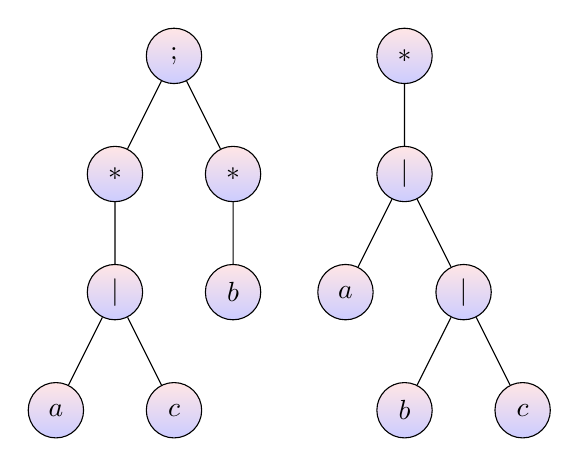
\begin{tikzpicture}[every node/.style = {shape=circle,
    draw, align=center,
    top color=red!10, bottom color=blue!20}]]
\usetikzlibrary{trees,chains}
\begin{scope}[start chain=growing right,minimum size=2em]
\node[on chain,circle,draw]{$;$} child {node{$*$} child{ node{$|$}  child{ node{$a$} } child{ node{$c$} }}}
 child{ node{$*$} child{ node{$b$}}};
\node[on chain,circle,draw,xshift=8ex]{$*$}
child {node{$|$}
child {node{$a$}}
child {node{$|$} child{ node{$b$}}  child{ node{$c$}}}
}
;
\end{scope}
\end{tikzpicture}
\section{הגלעין של שפת ליספ}
\newcommand{\TopAlign}[1]{\adjustbox{valign=t}{#1}}
\newcolumntype{T}{>{\collectcell{\TopAlign}}c<{\endcollectcell}}
%%%%%%%%%%%%%%%%%%%%%%%%%%%%%%%%%%%%%%%%%%%%%%%%%%%%%%%%%%%%%%%%%%%%%%%%%%%%%%%
% Code for collecting code exerpts into a separate library and kernel files
%%%%%%%%%%%%%%%%%%%%%%%%%%%%%%%%%%%%%%%%%%%%%%%%%%%%%%%%%%%%%%%%%%%%%%%%%%%%%%%
\newcounter{kernel}
\newcounter{library}
\setcounter{library}0

\newread \tempFile % A temporary reading stream
\newwrite \kernelFile % A stream to save kernel functions
\newwrite \libraryFile % A stream to save library functions
\immediate \openout \kernelFile=\jobname.kernel.lisp
\immediate \openout \libraryFile=\jobname.library.lisp

% An environment for writing kernel functions
\newenvironment{KERNEL}{%
  \stepcounter{kernel}
  \def\fileName{\jobname.kernel.\arabic{kernel}.lisp}%
  \global\let\savedifeof=\ifeof
  \def\ifeof##1{\global\let\ifeof=\savedifeof\iftrue}%
  \csname filecontents*\endcsname{\fileName}%
}{%
  \csname endfilecontents*\endcsname%
  \pagebreak[3]%
  \LTR
  \lstinputlisting[language=Mini,style=display,backgroundcolor=\color{olive!10}]{\fileName}%
  \endLTR
  \pagebreak[3]%
  \openin\tempFile=\fileName
  \begingroup\endlinechar=-1%
  \loop\unless\ifeof \tempFile
  \read\tempFile to\fileline % Read one line and store it into \fileline
  \immediate\write\kernelFile {\unexpanded\expandafter{\fileline}}%
  \repeat
  \immediate\write \kernelFile {¢}%
  \immediate\write \kernelFile {\unexpanded\expandafter{\pagebreak}[3]}%
  \immediate\write \kernelFile {¢}%
  \endgroup
  \closein \tempFile
}

% An environment for writing library functions
\newenvironment{LIBRARY}{%
  \stepcounter{library}
  \def\fileName{\jobname.library.\arabic{library}.lisp}%
  \global\let\savedifeof=\ifeof
  \def\ifeof##1{\global\let\ifeof=\savedifeof\iftrue}%
  \csname filecontents*\endcsname{\fileName}%
}{%
  \csname endfilecontents*\endcsname%
  \pagebreak[3]%
  \LTR
  \lstinputlisting[language=Mini,style=display,backgroundcolor=\color{orange!20}]{\fileName}%
  \endLTR
  \pagebreak[3]%
  \newread \tempFile % open the file to read from
  \openin \tempFile=\fileName
  \begingroup\endlinechar=-1
  \loop\unless\ifeof \tempFile
  \read\tempFile to\fileline % Read one line and store it into \fileline
  \immediate\write \libraryFile
  {\unexpanded\expandafter{\fileline}} % print the content to copy.txt
  \repeat
  \endgroup
  \closein \tempFile
}%



{%
    \makeatletter
    \catcode13=13\relax% Make ASCII 13 active to define it later
    \gdef\fixNewLine{%
        \def^^M{\space}%
    }%
}
§ מבוא
%\input lisp-aa

§ ביטויי~\E|S|
\תגית|פרק:S|
\input lisp-S

§עצי שיערוך ועצי דקדוק אבסטרקטי
%\input lisp-trees

§ מדריך למיני-ליספ 
\תגית|פרק:מיני|
%\input lisp-tutorial

§ מפרט של מיני-ליספ
%\input lisp-specification

§ אלגוריתם השיערוך ומימושו במיני-ליספ 
%\input lisp-evaluation-S-self
\תגית|פרק:שיערוך|

§ תרגילים
%\input lisp-exercises

\end{document}
